
%%%%%%%%%%%%%%%%%%%%%%%%%%%%%%%%%%%%%%%%%%%%%%%%%%%%%%%%%%%%%%%%%%%%%%%%%%%%%%%%
%%%%%%%%%%%%%%%%%%%%%%%%%%%%%%%%%%%%%%%%%%%%%%%%%%%%%%%%%%%%%%%%%%%%%%%%%%%%%%%%
\section{\textcolor{red}{Dançando no tempo e em contratempo}}
\index{Musicalidade!Dançando no tempo}
\index{Musicalidade!Dançando em contratempo}


Que significa dançar no tempo forte? 
pisar o tum  no tempo forte.

Se percebo que estou pisando no fraco como corrigir?
podemos usar
\begin{itemize}
\item Caminhada em contratempo
\item Fazemos balaços um número impar de vezes.
\end{itemize}


A Figura \ref{fig:tempovscontratempo}.

\begin{figure}[h]
    \centering 
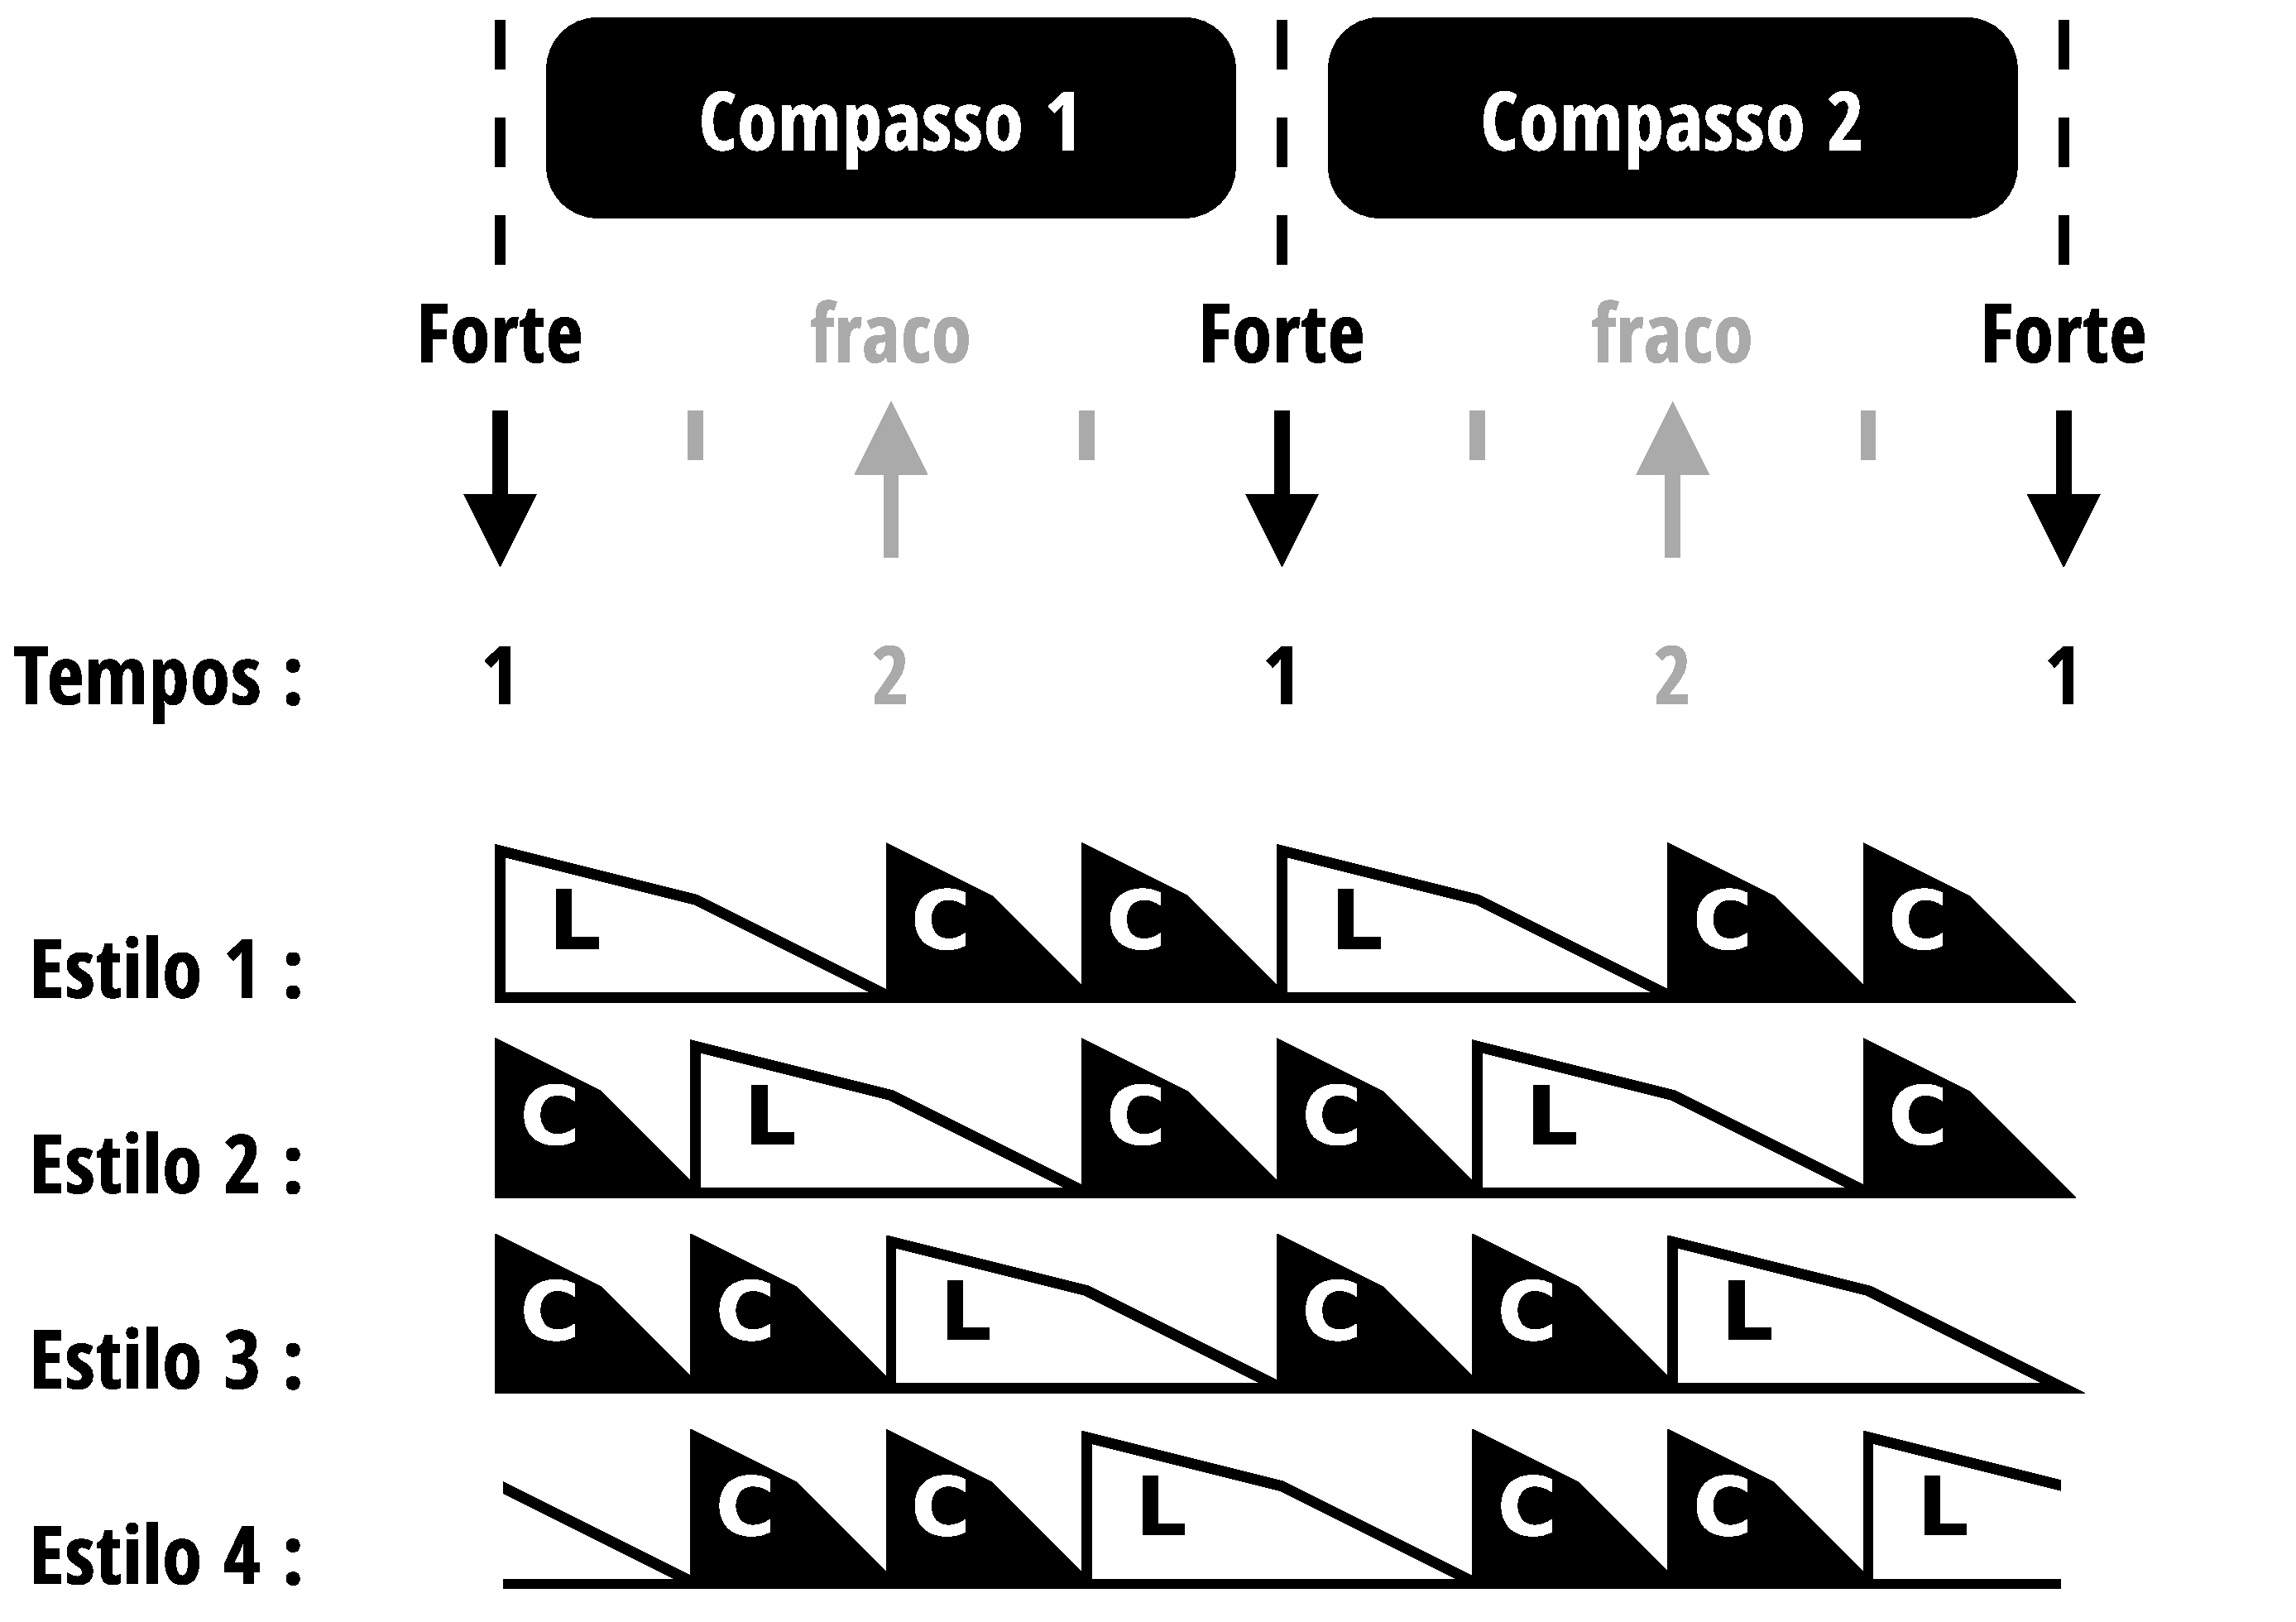
\includegraphics[width=0.9\textwidth]{chapters/cap-musicalidade/bailarcontratempo.eps}
    \caption{Percebendo métrica}\label{fig:tempovscontratempo}
\end{figure}
